\section{Appendices}
%%%%%%% SUPERVISOR MEETINGS %%%%%%%%
%%%%%%% SUPERVISOR MEETINGS %%%%%%%%
%%%%%%% SUPERVISOR MEETINGS %%%%%%%%
%%%%%%% SUPERVISOR MEETINGS %%%%%%%%
%%%%%%% SUPERVISOR MEETINGS %%%%%%%%

\subsection{Semester 2 Supervisor Meetings}

\begin{table}[H]
	\centering
	\begin{tabular}{|l|l|l|}
		\hline
		\multicolumn{3}{|c|}{\textbf{2017 Supervisor Meeting Summary}}                                                                                                                                                                                                                              \\ \hline
		\textit{Date} & \textit{Time} & \textit{Discussion Points}                                                                                                                                                                                                                                  \\ \hline
		31 Jan 2017   & 1200-1230     & \begin{tabular}[c]{@{}l@{}}- Feedback from 2016 reports\\ - Research shortcomings\\ \\ - My plan for remaining tasks\\ - Explained where I was wrong with terminology\end{tabular}                                                                          \\ \hline
		17 Apr 2017   & 1300-1400     & \begin{tabular}[c]{@{}l@{}}- Report structure changes\\ - Different PV calculation techniques\\ - Necessary additions to PV section\\ - Incorrect assumptions during calculation\\ - Discussed remaining tasks\\ - Discussed oral presentation\end{tabular} 
		\\ \hline
		9 May 2017   & 1200-1400     & \begin{tabular}[c]{@{}l@{}}- Checked over full report\\ - Received grade for progress report 2\\ - Agreed on remaining tasks\\ - Discussed presentation requirements\\ - Provided tips on technical writing\\ - Provide guidance final building model\end{tabular} 
		\\ \hline
	\end{tabular}
	\caption{Supervisor Meetings of 2017 Summary}
	\label{table:supervisor-meeting-summary}
\end{table}

\newpage

%%%%%%% TIMELINE %%%%%%%%
%%%%%%% TIMELINE %%%%%%%%
%%%%%%% TIMELINE %%%%%%%%
%%%%%%% TIMELINE %%%%%%%%
%%%%%%% TIMELINE %%%%%%%%
%%%%%%% TIMELINE %%%%%%%%
%%%%%%% TIMELINE %%%%%%%%
%%%%%%% TIMELINE %%%%%%%%


\subsection{Timeline Analysis} \label{appendix:Timeline}

\paragraph{}
The tasks were be split into days and University weeks. It was ensured to include the holidays during periods where University is not run. This project does not simply end upon the completion of this semester. BEB801 is concluded on November 4th at the end of Week 14, however BEB802 is the subject allocation to complete the second half of this project. The task table will allocate SMART milestones. Additionally, the benefits of completing the subjects during this period is that there is the additional time from summer holidays to account for.

\paragraph{}
Table \ref{table:timeline_original} on the following page shows the milestones of this project. The University assigned submissions are represented as bold text. The four major deliverables for the first half of this project are the library assessment, project proposal, oral presentation and progress report. These four deliverables are what have outlined how the remaining tasks have been created and the time periods allowed for. Earlier due dates are set to allow for editing or possible difficulties to occur without major repercussions. 

\paragraph{}
Table \ref{table:timeline_revised} represents the revised timeline with completed times. This is for the benefit of both the creator of this project as well as any future students who wish to progress the project and extend its scope. There are a variety of reasons as to why there were extensions of time for completing milestones. It is not an irregular occurrence that project plans are extended and this project is no different. As previously discussed, deadlines were set at least 1 week early with the intention of ensuring proper preparation is done and deadlines are not missed.     

\newpage
\textbf{Initial Timeline}

% Table of Tasks
\begin{table}[H]
	\centering
	\begin{tabular}{||c c||} 
		\hline
		\multicolumn{2}{|c|}{\textbf{Initial Project Timeline}} \\ [0.5ex] 
		\hline\hline
		\textbf{Milestone} & \textbf{Deadline} \\ 
		\hline\hline
		Project Definition 							& Sem 1 Week 3 \\ 
		\textbf{Library Assessment} 				& \textbf{Sem 1 Week 4} \\
		Initial Research Phase 						& Sem 1 Week 6 \\
		\textbf{Project Proposal} 					& \textbf{Sem 1 Week 7} \\
		Initial Design Phase 						& Sem 1 Week 9 \\
		Initial Prototype Design Finalised 			& Sem 1 Week 11 \\
		Initial 3D Modelling for Presentation 		& Sem 1 Week 12 \\
		\textbf{Initial Oral Presentation} 			& \textbf{Sem 1 Week 14} \\ 
		\textbf{Written Report} 					& \textbf{Sem 1 Week 14} \\ 
		Implement Feedback From Report 				& Summer Break \\
		Complete Research Shortcomings 				& Summer Break \\
		Complete Further Technical Calculations 	& Summer Break \\
		Initial Finance Analysis 					& Sem 2 Week 2 \\
		Design Simulations 							& Sem 2 Week 6 \\
		\textbf{Progress Report} 					& \textbf{Sem 2 Week 7} \\
		Finalised Design 							& Sem 2 Week 10 \\
		Finalised Simulations \& 3D Modelling 		& Sem 2 Week 11 \\
		Finalised Financial Analysis				& Sem 2 Week 12 \\
		\textbf{Final Presentation} 				& \textbf{Sem 2 Week 14} \\
		\textbf{Final Report} 						& \textbf{Sem 2 Week 14} \\ [1ex] 
		\hline
	\end{tabular}
	\caption{Initial Project Timeline}
	\label{table:timeline_original}
\end{table}    

\newpage
\textbf{Revised Timeline}

% Table of Tasks
\begin{table}[H]
	\centering
	\begin{tabular}{||p{5cm} c c||} 
		\hline
		\textbf{Milestone} & \textbf{Original Deadline} & \textbf{Actual Completion} \\ [0.5ex] 
		\hline\hline
		Project Definition 							& Week 3 			& Week 3\\ 
		\textbf{Library Assessment} 				& \textbf{Week 4} 	& Week 4\\
		Initial Research Phase 						& Week 6 			& Week 6\\
		\textbf{Project Proposal} 					& \textbf{Week 7} 	& Week 7\\
		Initial Design Phase 						& Week 9			& Week 10\\
		Initial Prototype Design Finalised 			& Week 11 			& NA\\
		Initial 3D Modelling for Presentation 		& Week 12 			& Week 11\\ 
		\textbf{Initial Oral Presentation} 			& \textbf{Week 14} 	& Week 14\\
		\textbf{Written Report} 					& \textbf{Week 14} 	& Week 14\\ 
		Implement Feedback From Report 				& Summer Break 		& Summer Break \\
		Complete Research Shortcomings 				& Summer Break 		& Summer Break \\
		Complete Further Technical Calculations 	& Summer Break 		& Week 8 \\
		Initial Finance Analysis 					& Week 2 			& TBC \\
		Design Simulations 							& Week 6 			& Week 8 \\ 
		\textbf{Progress Report} 					& \textbf{Week 8} 	& Week 8 \\
		Finalised Design 							& Week 10 			& TBC \\
		Finalised Simulations \& 3D Modelling 		& Week 11 			& TBC \\
		Finalised Financial Analysis 				& Week 12 			& TBC \\ 
		\textbf{Final Presentation} 				& \textbf{Week 14} 	& TBC\\
		\textbf{Final Report} 						& \textbf{Week 14} 	& TBC\\ [1ex] 
		\hline
	\end{tabular}
	\caption{Initial Project Timeline Analysis}
	\label{table:timeline_revised}
\end{table}      

%%%%%%% PROJECT DRAFT MODEL %%%%%%%%
%%%%%%% PROJECT DRAFT MODEL %%%%%%%%
%%%%%%% PROJECT DRAFT MODEL %%%%%%%%
%%%%%%% PROJECT DRAFT MODEL %%%%%%%%
%%%%%%% PROJECT DRAFT MODEL %%%%%%%%


\subsection{Draft Floor Plan} \label{section:draft-floor-plan}

%New Paragraph
Before the schematics and floor plans for QUT's buildings were made available, an approximate small office area was modelled in AutoCAD with offices of 5\si{m^2} represented in Figure \ref{fig:RoughFloorplan}. The purpose of this simulation was to analyse approximate lighting loads for the environment. It was only used as a preliminary design approximation until more time was allocated to design.  

\begin{figure}[H]
	\hfill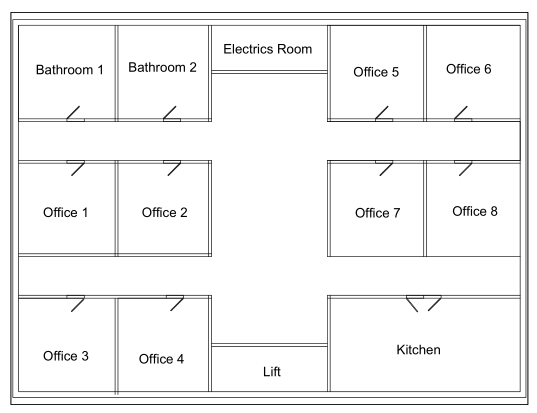
\includegraphics[width = 100mm]{images/Rough_Floorplan}\hspace*{\fill}
	\caption{Initial Draft Floor Plan Design} 
	\label{fig:RoughFloorplan}
\end{figure} 

\subsubsection{Draft Floor Plan Lighting Simulation}

%New Paragraph
After the initial room plans were created, the Australian Standards AS/NZS 1680.2.2 Interior and Workplace Lighting were consulted to produce a table of required lux values depending on room use. The standards is replicated and simplified below in Table \ref{table:LightingRequirements}.

\begin{table}[H]
	\centering
	\renewcommand{\arraystretch}{2}
	\begin{tabular}{|l|c|}
		\hline
		\textbf{Area or Application} 	& \textbf{Lux Requirement} \\ \hline
		Rarely Visited 					& 40 \\ \hline
		Storage Rooms or Change Room 	& 80 \\ \hline
		Machine Work or Waiting Room 	& 160 \\ \hline
		Food Preparation Room 			& 240 \\ \hline
		Technical Office Room 			& 320 \\ \hline
		Visually Difficult Work 		& 500 \\ \hline
	\end{tabular}
	\caption{Lighting Requirements as per AS/NZS Standards \cite{StandardsAustralia2006_2}}
	\label{table:LightingRequirements}
\end{table}

These two data points were used for the initial draft planning of designs. This is not an accurate representation of a building, it was a starting point to work from to beginning analysis load requirements. Once the more accurate schematics and plans are created, a stronger assessment can be created and feasibly power system construction plans created. To estimate load requirements for this smaller, draft area, the simple floor plan CAD file was imported into Dialux4.13. This is a lighting design software solution to model options and predict approximate load demands that the LVDC system will be required to power.  
\newline

%New Paragraph
Through personal experience in building services design, I had an approximate idea of what amounts of lighting would be required for a 5\,\si{m^2} room. I also knew that I would use LED down lights for simplicity and affordability. The difficult part is finding commercially available products that operate at a voltage level at either 48 V DC when the voltage drop over cabling is removed or at another level where an efficient DC to DC converter could be used. My goal was to have the average lux between 300\,\si{lux} to 400\,\si{lux}. This value was chosen as a technical office is an accurate assessment of most corporate buildings. As seen in Table \ref{table:draftFloorPlanDialuxOutputs} below, seven 20\,\si{W} LED down lights reaches this specification. The way this was completed was through multiple tested and rendering of designs. It can be a tedious process but photometric files (also known as IES files) are also imported into Dialux and can be placed throughout the 3D model. This 3D model is shown in Figure \ref{fig:DraftLighting3D}. To find the optimal solution, the simplest method is to remove and add lights of varying wattage and test the lux distribution. An example of the lux distribution is shown in Figure \ref{fig:DraftLightingLux}. Appendix \ref{appenddix:DraftFloorPlanLighting} shows the full report of the final working model.   

\begin{table}[!ht]
	\centering
	\renewcommand{\arraystretch}{1}
	\begin{tabular}{|c|c|c|c|c|}
		\hline
		\multicolumn{1}{|l|}{\textbf{Down Light Wattage}} & \multicolumn{1}{l|}{\textbf{Quantity}} & \multicolumn{1}{l|}{\textbf{Max Lux}} & \multicolumn{1}{l|}{\textbf{Min Lux}} & \multicolumn{1}{l|}{\textbf{Average Lux}} \\ \hline
		11 & 6 & 114 & 3.8 & 73 \\ \hline
		11 & 10 & 180 & 7 & 114 \\ \hline
		20 & 8 & 680 & 16 & 383 \\ \hline
		20 & 7 & 677 & 12 & 344 \\ \hline
	\end{tabular}
	\caption{Dialux Outputs of Initial Draft Floor Plan}
	\label{table:draftFloorPlanDialuxOutputs}
\end{table} 

\begin{figure}[H]
	\hfill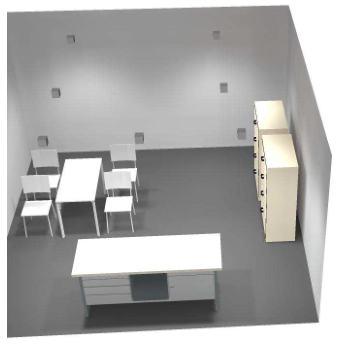
\includegraphics[width = 100mm]{images/lighting_draft_3D}\hspace*{\fill}
	\caption{Initial Draft Floor Plan Lighting Test 3D Render} 
	\label{fig:DraftLighting3D}
\end{figure} 

\begin{figure}[H]
	\hfill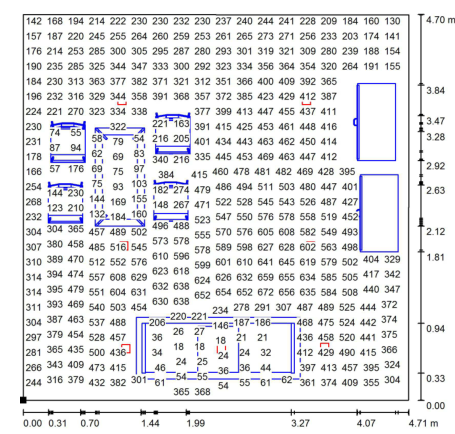
\includegraphics[width = 100mm]{images/lighting_draft_output}\hspace*{\fill}
	\caption{Initial Draft Floor Plan Lighting Test Lux Output} 
	\label{fig:DraftLightingLux}
\end{figure} 

%New Paragraph
Continuing from this example, the total lighting load of an office room would therefore be 140 W (20\,W * 7 lights). To approximate the total demand for the entire draft floor plan, there are bathrooms, kitchen and hallways that all require less light. If the offices' load is approximately 1.1 kW it can be expected that the total area lighting load would approach 1.8 kW. This is a good starting point and more accurate modelling can now be done with QUT's provided power data. 




%%%%%%% LEVEL 7 MARKUP %%%%%%%%
%%%%%%% LEVEL 7 MARKUP %%%%%%%%
%%%%%%% LEVEL 7 MARKUP %%%%%%%%\\
%%%%%%% LEVEL 7 MARKUP %%%%%%%%\\
%%%%%%% LEVEL 7 MARKUP %%%%%%%%\\

\newpage

\subsection{QUT P Block Level 6 Office Markup}
\label{appendix:qut_lvl6_markup}
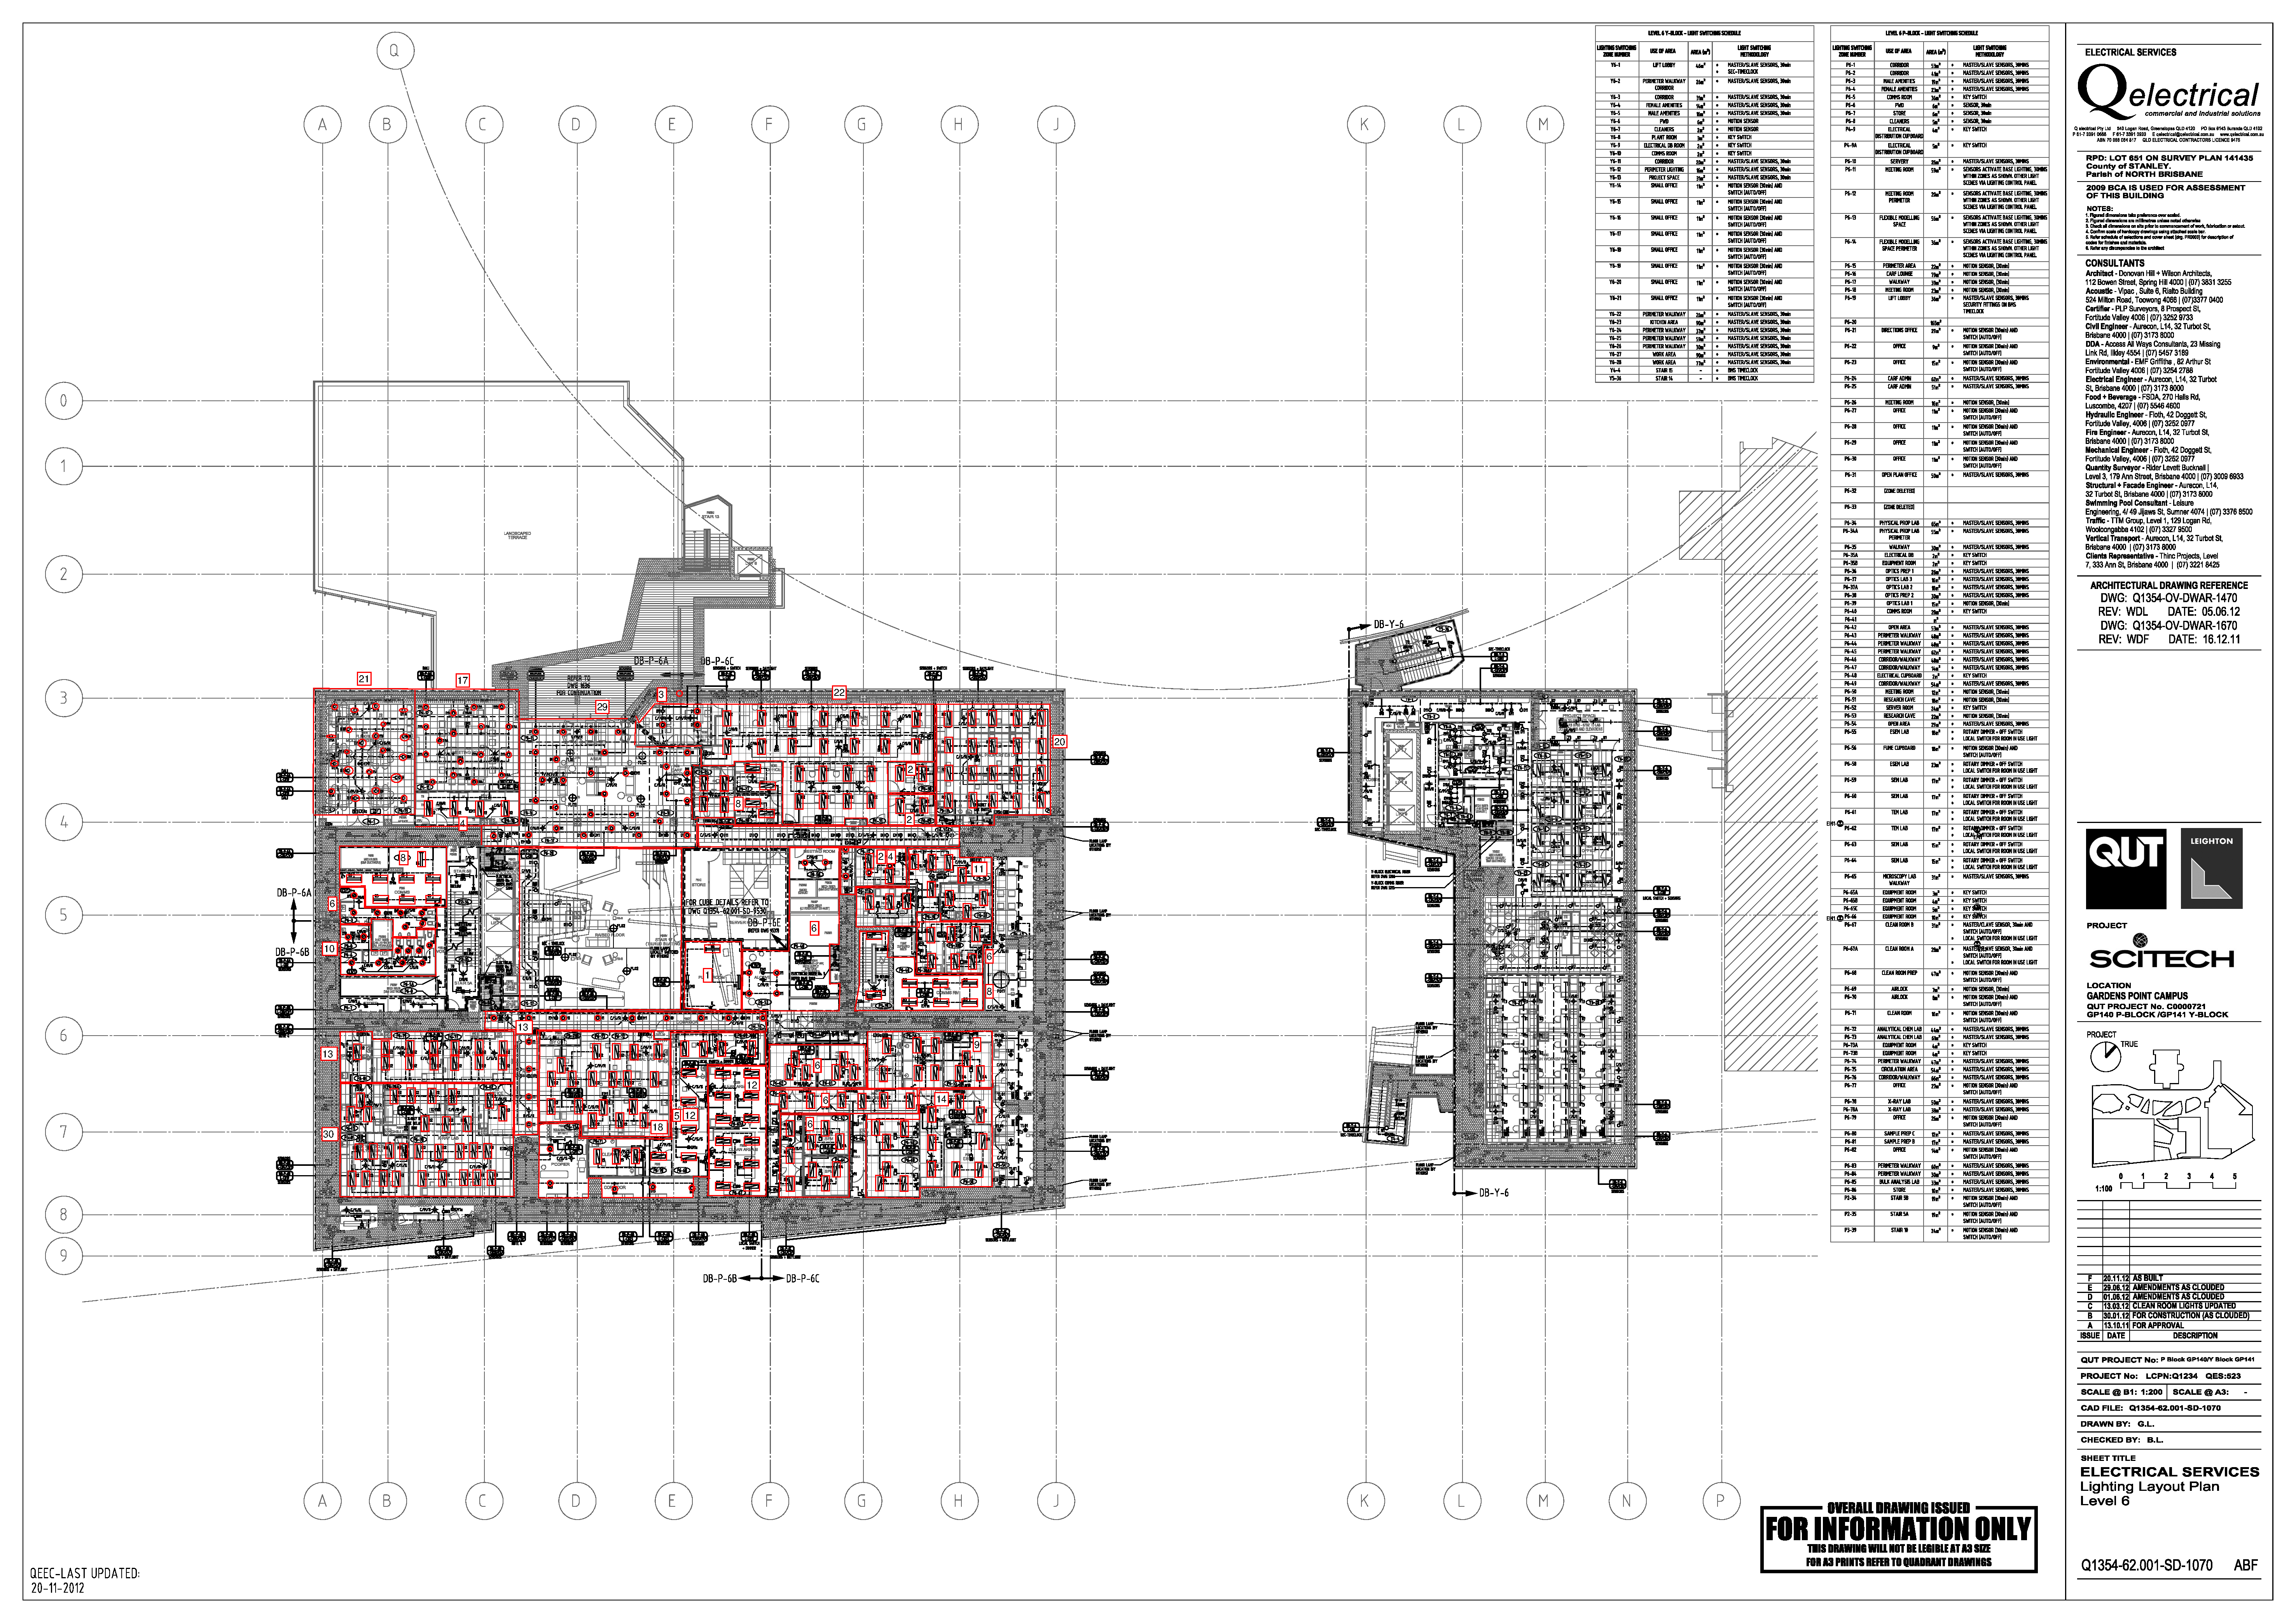
\includepdf[pages={1},angle=-90]{appendix/qut_lvl6_markup}

%%%%%%%%%%%%%%%
%							LEVEL 6 OFFICE LIGHITNG SIMULATION
%%%%%%%%%%%%%%%

\subsection{QUT P Block Level 6 Office Lighting Simulation}
\label{appendix:QUT-Lvl6-office-rev3}
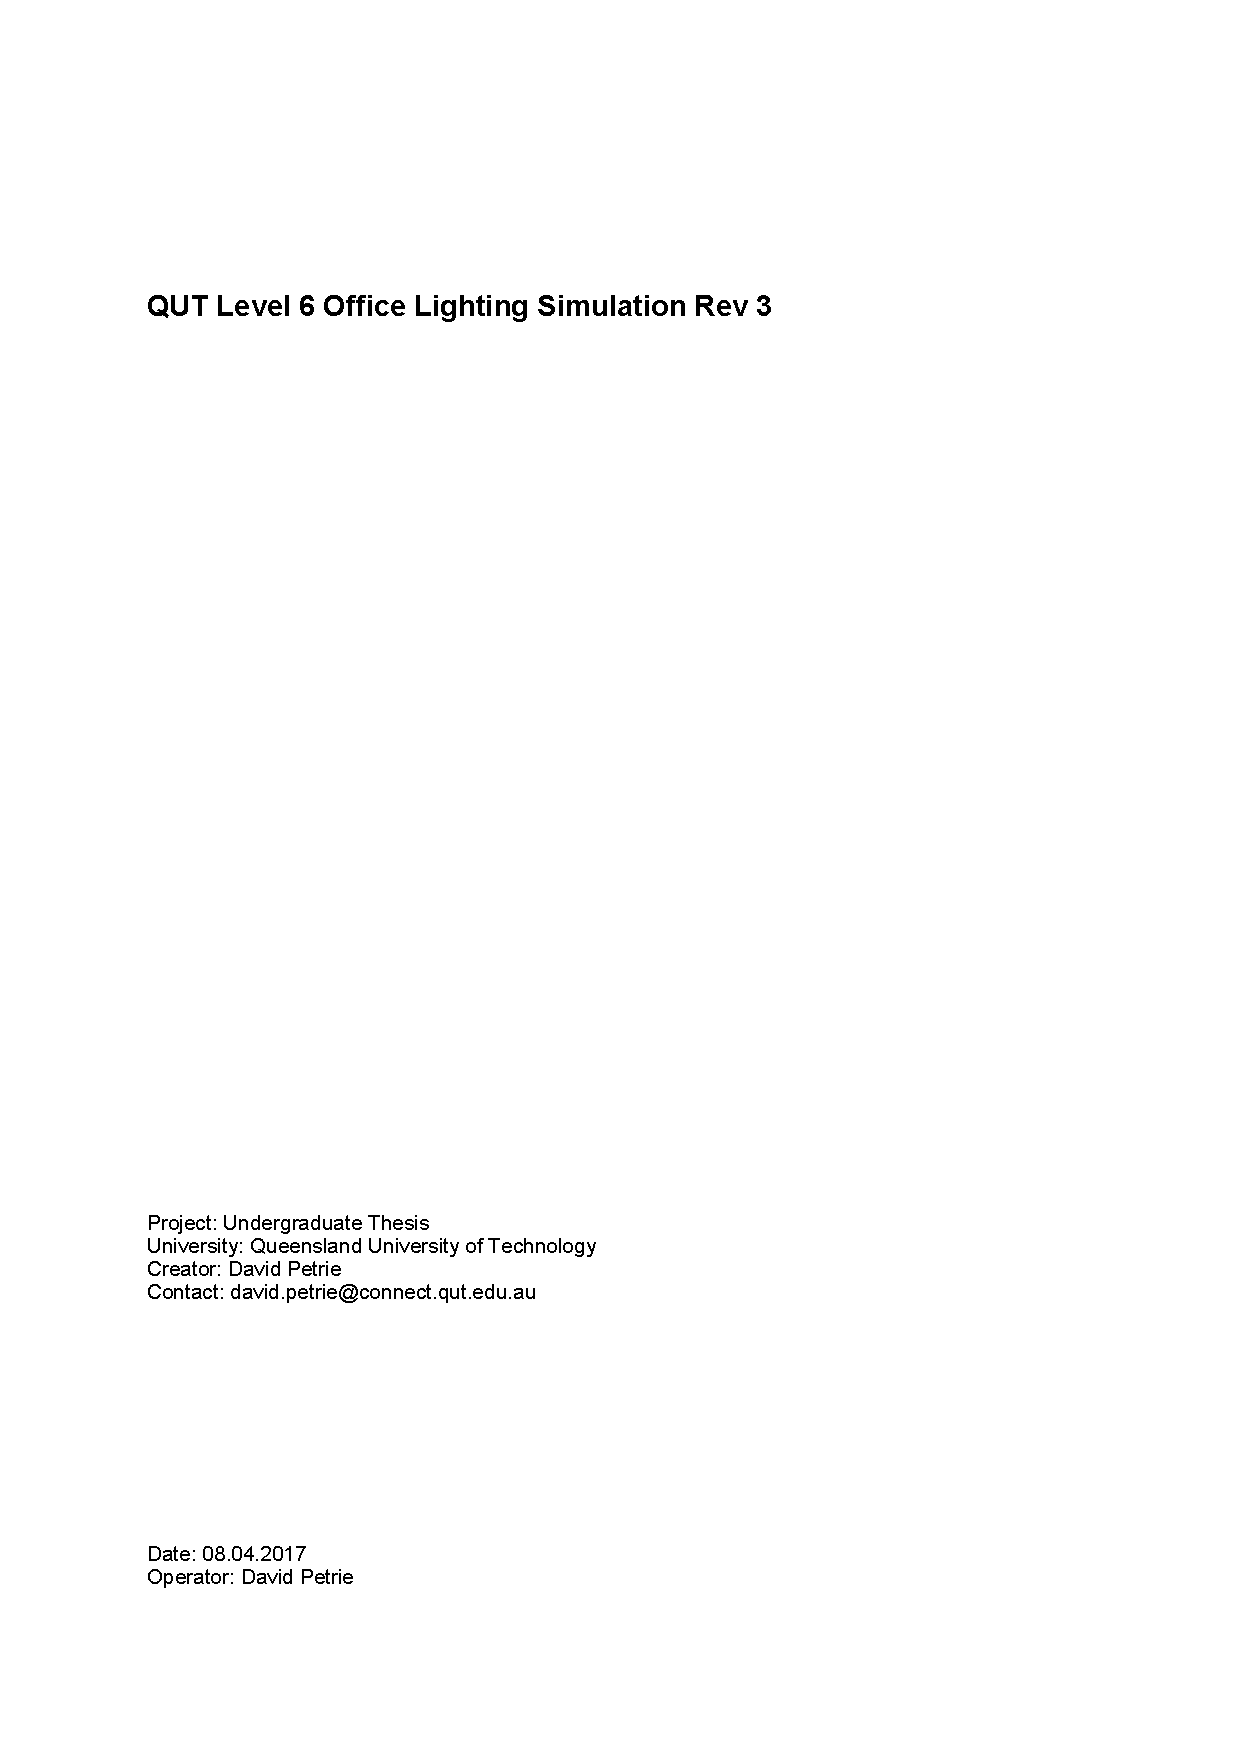
\includepdf[pages={1-8}]{appendix/QUT-Lvl6-office-rev3.pdf}

%%%%%%%%%%%%%%%
%							DRAFT FLOORPLAN DIALUX REPORT
%%%%%%%%%%%%%%%

\subsection{Draft Floor Plan Lighting Analysis Report}
\label{appenddix:DraftFloorPlanLighting}
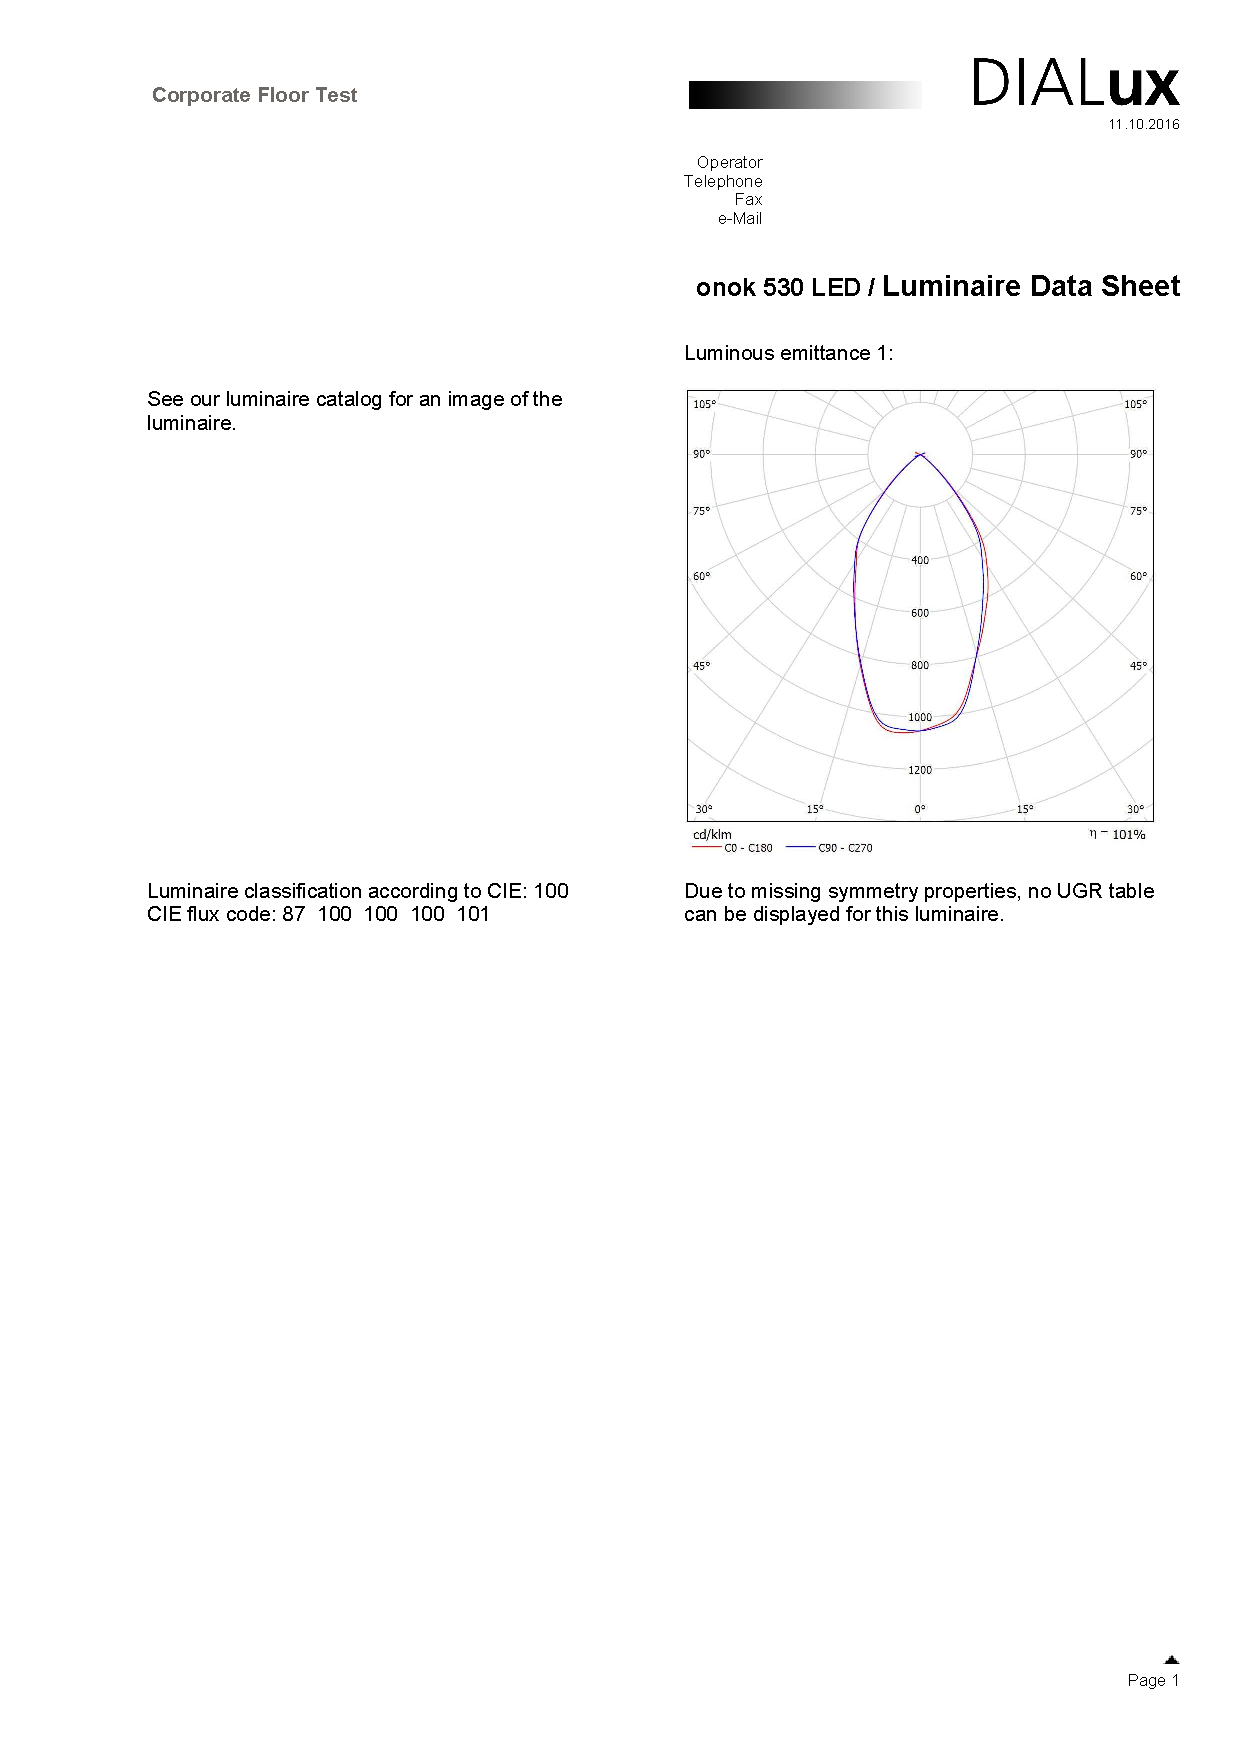
\includepdf[pages={1-12}]{appendix/draft_light_report.pdf}


